\documentclass[hidelinks,12pt,dvipsnames,border=2pt]{standalone}
%\usepackage[top=0.7in, bottom=0.8in, left=1in, right=1in]{geometry}
\usepackage{tikz}
\usepackage{hyperref}
\usetikzlibrary{arrows}
\usetikzlibrary{shapes}
\usepackage{enumitem}
\usepackage{bm}
\usepackage{mathdots}
\usepackage{amsmath}
\usetikzlibrary{shadings}
\usetikzlibrary{decorations.pathreplacing}
\usepackage{helvet}
\usepackage{url}
\usepackage{graphicx}
\usetikzlibrary{arrows.meta,positioning,fit,calc}
\renewcommand{\familydefault}{\sfdefault}


\usetikzlibrary{arrows,decorations.pathmorphing,backgrounds,fit,positioning,shapes.symbols,chains}

\begin{document}
	
	
% trim=left botm right top
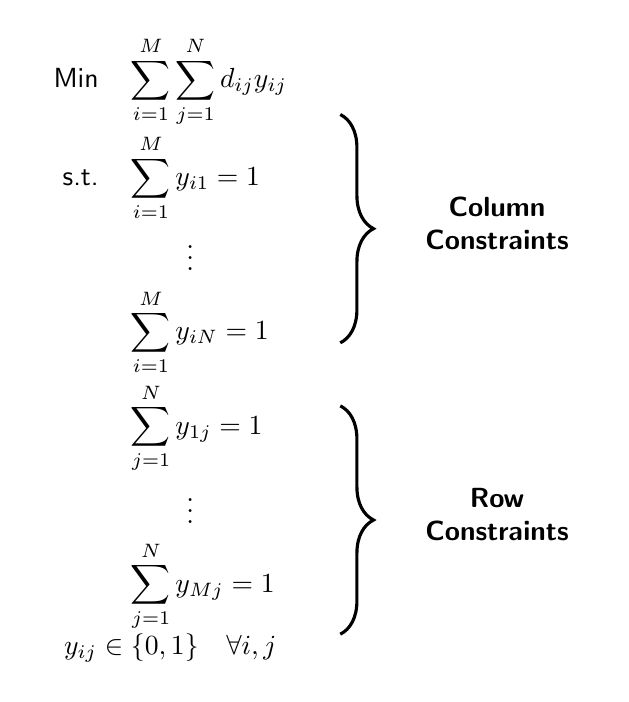
\begin{tikzpicture}
\node at (0,0) {
	\begin{tabular}{c}
		{$\begin{aligned}
			\text{Min} \quad  & \sum_{i = 1}^{M} \sum_{j = 1}^{N} d_{ij} y_{ij} \\
			\text{s.t.} \quad & \sum_{i = 1}^{M} y_{i1} = 1 \\
			& \quad \quad \vdots \\
			& \sum_{i = 1}^{M} y_{iN} = 1 \\
			& \sum_{j = 1}^{N} y_{1j} = 1 \\
			& \quad \quad \vdots \\
			& \sum_{j = 1}^{N} y_{Mj} = 1 \\
	    \end{aligned}$} \\ [20ex]
    $y_{ij} \in \{0,1\} \quad \forall i,j$
	    \end{tabular}
};

\draw [decorate,decoration={brace,amplitude=12pt,aspect=0.5,mirror},xshift=-4pt,yshift=0pt,line width=0.4mm] (2.3,0.1) -- (2.3,3) node [black,xshift=9pt] {\footnotesize};
\node[text width=2.4cm] at (4.15,1.55) {\vspace{-0.6cm}\begin{center}\textbf{Column Constraints}\end{center}};

\draw [decorate,decoration={brace,amplitude=12pt,aspect=0.5,mirror},xshift=-4pt,yshift=0pt,line width=0.4mm] (2.3,-3.6) -- (2.3,-0.7) node [black,xshift=9pt] {\footnotesize};
\node[text width=2.4cm] at (4.15,-2.15) {\vspace{-0.6cm}\begin{center}\textbf{Row Constraints}\end{center}};
\end{tikzpicture}

\end{document}